\documentclass[a4paper,12pt]{article}
\usepackage{fontspec}
\usepackage{xeCJK}
\usepackage{amsmath}
\usepackage{amsthm}
\usepackage{amsfonts}
\usepackage{amssymb}
\usepackage{graphicx}
\usepackage{hyperref}
\usepackage{enumitem}
\usepackage{textcomp}
\usepackage{float}
\usepackage{booktabs}
\usepackage{url}
\usepackage[left=1.50cm, right=1.50cm, top=1.20cm]{geometry}
\linespread{1.5}
\usepackage{algorithm}
\usepackage{algpseudocode}
\usepackage[tikz]{mdframed}
\usetikzlibrary{matrix, positioning, fit, arrows, calc, intersections, shapes, shadings, patterns, decorations.markings, chains, scopes, shapes.arrows}
\usepackage{upquote}
\usepackage{tikzpeople}
\usepackage{tikzsymbols}
\usepackage{listings}
\usepackage{color}
\usepackage{logicpuzzle}
\usepackage{subcaption}
\usepackage[tikz]{mdframed}
\lstdefinestyle{customc}{
  belowcaptionskip=1\baselineskip,
  breaklines=true,
  frame=L,
  xleftmargin=\parindent,
  language=C++,
  tabsize=2,
  %numbers=left,
  %stepnumber=1,
  showstringspaces=false,
  basicstyle=\small\ttfamily,
  keywordstyle=\bfseries\color{green!40!black},
  commentstyle=\itshape\color{purple!40!black},
  identifierstyle=\color{blue},
  stringstyle=\color{orange},
}
\mdfdefinestyle{mymdf}{leftmargin=1cm,rightmargin=2cm,%
innerleftmargin=1cm,innerrightmargin=1cm,roundcorner=10pt,backgroundcolor=lg}
\definecolor{lg}{RGB}{247,249,250}
\title{Algorithm Problem Set \\ \large No. 800 --- 899}
\author{SS}

\begin{document}
\renewcommand{\thelstlisting}{\thesection.\arabic{lstlisting}}
\newcommand{\fcc}[1]{\lstinline[language=C++, basicstyle=\small\ttfamily, keywordstyle=\bfseries\color{green!40!black}]|#1|}
\newcommand{\fcj}[1]{\lstinline[language=Java, basicstyle=\small\ttfamily, keywordstyle=\bfseries\color{green!40!black}]|#1|}
%\sloppy
\maketitle
\section{800 --- Similar RGB Color}
In the following, every capital letter represents some hexadecimal digit from 0 to f.

The red-green-blue color \fcj{"#AABBCC"} can be written as \fcj{"#ABC"} in shorthand.  For example, \fcj{"#15c"} is shorthand for the color \fcj{"#1155cc"}.

Now, say the similarity between two colors \fcj{"#ABCDEF"} and \fcj{"#UVWXYZ"} is 

\fcj{-(AB - UV)^2 - (CD - WX)^2 - (EF - YZ)^2}.

Given the color \fcj{"#ABCDEF"}, return a 7 character color that is most similar to \fcj{#ABCDEF}, and has a shorthand (that is, it can be represented as some \fcj{"#XYZ"}

\paragraph{Example 1:}

\begin{flushleft}
\textbf{Input}: \fcj{color = "#09f166"}

\textbf{Output}: \fcj{"#11ee66"}

\textbf{Explanation}:  

The similarity is \fcj{-(0x09 - 0x11)^2 -(0xf1 - 0xee)^2 - (0x66 - 0x66)^2 = -64 -9 -0 = -73}.

This is the highest among any shorthand color.
\end{flushleft}

\paragraph{Note:}

\begin{itemize}
\item \fcj{color} is a string of length 7.
\item \fcj{color} is a valid RGB color: for \fcj{i > 0}, \fcj{color[i]} is a hexadecimal digit from 0 to f
\item Any answer which has the same (highest) similarity as the best answer will be accepted.
\item All inputs and outputs should use lowercase letters, and the output is 7 characters.
\end{itemize}

\subsection{Brute Force}
Each digit in the shorthand \fcj{"#RGB"} could be from 0 to 15. This leads to a color of 
\fcj{17 * R * (1 << 16) + 17 * G * (1 << 8) + 17 * B}. 

The reason for the 17 is because a hexadecimal value of \fcj{0x22} is equal to \fcj{2 * 16 + 2 * 1} which is \fcj{2 * (17)}. The other values for red and green work similarly, just shifted up by 8 or 16 bits.

It should be noted that the answer is always unique. Indeed, for two numbers that differ by 17, every integer is closer to one than the other. For example, with 0 and 17, 8 is closer to 0 and 9 is closer to 17 --- there is no number that is tied in closeness.

\setcounter{lstlisting}{0}
\begin{lstlisting}[style=customc, caption={Brute Force}]
string similarRGB( string color )
{
    for( size_t i = 1; i < color.size(); i += 2 )
    {
        //change to integer
        auto num = stoi( color.substr( i, 2 ), nullptr, 16 );
        //get the closet integer with form (cc)
        int x = num / 17 + ( ( num % 17 ) > 8 ? 1 : 0 );
        //change to string
        color[i] = ( x > 9 ) ? ( x - 10 + 'a' ) : ( x + '0' );
        color[i + 1] = color[i];
    }

    return color;
}
\end{lstlisting}
\section{801 --- Minimum Swaps To Make Sequences Increasing}

\textbf{Medium}

We have two integer sequences A and B of the same non-zero length.

We are allowed to swap elements \fcj{A[i]} and \fcj{B[i]}.  Note that both elements are in the same index position in their respective sequences.

At the end of some number of swaps, A and B are both strictly increasing. (A sequence is strictly increasing if and only if 

\fcj{A[0] < A[1] < A[2] < ... < A[A.length - 1]}. )

Given A and B, return the minimum number of swaps to make both sequences strictly increasing.  It is guaranteed that the given input always makes it possible.

\paragraph{Example:}

\begin{flushleft}
\textbf{Input}: \fcj{A = [1,3,5,4]}, \fcj{B = [1,2,3,7]}

\textbf{Output}: 1

\textbf{Explanation}: 

Swap A[3] and B[3].  Then the sequences are:

\fcj{A = [1, 3, 5, 7]} and \fcj{B = [1, 2, 3, 4]}

which are both strictly increasing.
\end{flushleft}

\paragraph{Note:}

\begin{itemize}
\item A, B are arrays with the same length, and that length will be in the range \fcj{[1, 1000]}.

\item \fcj{A[i]}, \fcj{B[i]} are integer values in the range \fcj{[0, 2000]}.
\end{itemize}

\subsection{Dynamic Programming}
Suppose $n_1$ is the cost of making the first $i-1$ columns increasing and not swapping the $(i-1)$th column; and $s_1$ is the cost of making the first $i-1$ columns increasing and swapping the $(i-1)$th column.

Now we want candidates $n_2$ (and $s_2$), the costs of making the first $i$ columns increasing if we do not swap (or swap, respectively) the $i$th column.

\paragraph{Algorithm}

Say $a_1 = A[i-1]$, $b_1 = B[i-1]$ and $a_2 = A[i]$, $b_2 = B[i]$.

Now, if $a_1 < a_2$ and $b_1 < b_2$, it is allowed to have both of these columns unswapped, or both of these columns swapped. This leads to $n_2 = \min(n_2, n_1)$ and $s_2 = \min(s_2, s_1 + 1)$.

Another possibility is that $ a_1 < b_2 $ and $ b_1 < a_2 $. This means that it is allowed to have exactly one of these columns swapped. This leads to $n_2 = \min(n_2, s_1)$ or $s_2 = \min(s_2, n_1 + 1)$.

Note that it is important to use two \fcj{if} statements separately, because both of the above possibilities might be possible.

At the end, the optimal solution must leave the last column either natural or swapped, so we take the minimum number of swaps between the two possibilities.


\setcounter{lstlisting}{0}
\begin{lstlisting}[style=customc, caption={Dynamic Programming}]
int minSwap( vector<int>& A, vector<int>& B )
{
    //n1 = the cost of making first (i-1) columns sorted
    //but not swap column (i-1)
    int n1 = 0;
    //s1 = the cost of making first (i-1) columns sorted
    //but swap column (i-1)
    int s1 = 1;

    for( size_t i = 1; i < A.size(); ++i )
    {
        int n2 = INT_MAX;
        int s2 = INT_MAX;
        if( ( A[i - 1] < A[i] ) && ( B[i - 1] < B[i] ) )
        {
            //we can choose to not swap column (i-1) and (i)
            n2 = ( min )( n2, n1 );
            //or we can choose to swap column (i-1) and (i)
            s2 = ( min )( s2, s1 + 1 );
        }

        if( ( A[i - 1] < B[i] ) && ( B[i - 1] < A[i] ) )
        {
            //we can choose to swap column (i-1)
            //but leave column i not swapped
            n2 = ( min )( n2, s1 );
            //or we can choose to swap column i
            //but leave column (i-1) not swapped
            s2 = ( min )( s2, n1 + 1 );
        }

        n1 = n2;
        s1 = s2;
    }
    //the minimum of n1 and s1 is the answer
    return ( min )( n1, s1 );
}
\end{lstlisting}

\section{802 --- Find Eventual Safe States}

\textbf{Medium}

In a directed graph, we start at some node and every turn, walk along a directed edge of the graph. If we reach a node that is terminal (that is, it has no outgoing directed edges), we stop.

Now, say our starting node is eventually safe if and only if we must eventually walk to a terminal node. More specifically, there exists a natural number K so that for any choice of where to walk, we must have stopped at a terminal node in less than K steps.

Which nodes are eventually safe?  Return them as an array in sorted order.

The directed graph has $N$ nodes with labels 0, 1, $\ldots$, $N-1$, where $N$ is the length of graph. The graph is given in the following form: \fcj{graph[i]} is a list of labels $j$ such that $ (i, j) $ is a directed edge of the graph.

\paragraph{Example:}
\begin{flushleft}


\textbf{Input}: \fcj{graph = [[1,2],[2,3],[5],[0],[5],[],[]]}

\textbf{Output}: \fcj{[2,4,5,6]}

Here is a diagram of the above graph.

\begin{figure}[H]
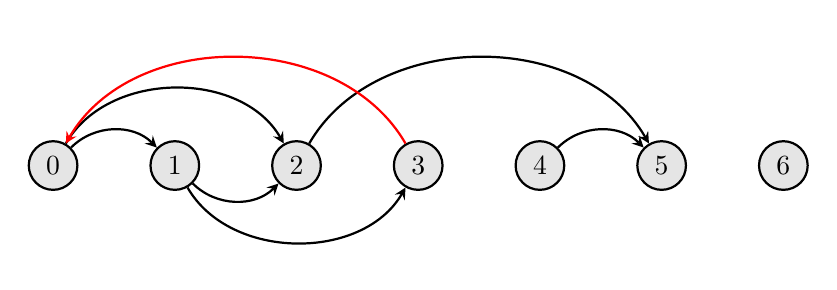
\begin{tikzpicture}
[every node/.style={draw, circle, fill=gray!20!, minimum size=5mm},
thick, ->, >=stealth, node distance=9mm, start chain]
\node(0)[on chain]{0};
\node(1)[on chain]{1};
\node(2)[on chain]{2};
\node(3)[on chain]{3};
\node(4)[on chain]{4};
\node(5)[on chain]{5};
\node(6)[on chain]{6};
\draw (0) to [bend left=45] (1);
\draw (0) to [bend left=60] (2);
\draw (1) to [bend right=45] (2);
\draw (1) to [bend right=60] (3);
\draw (2) to [bend left=60] (5);
\draw (4) to [bend left=45] (5);
\draw[red] (3) to [bend right=60] (0);
\end{tikzpicture}
\end{figure}

\end{flushleft}

\paragraph{Note:}

\begin{itemize}
\item \fcj{graph} will have length at most 10000.
\item The number of edges in the \fcj{graph} will not exceed 32000.
\item Each \fcj{graph[i]} will be a sorted list of different integers, chosen within the range \fcj{[0, graph.length - 1]}.
\end{itemize}

\subsection{Depth-First Search}
We can apply a classic \textit{white-gray-black} DFS algorithm by marking the node \textit{gray} on entry and \textit{black} on exit. If we see a \textit{gray} node during DFS, it must be part of a cycle.

For this problem, When we visit a node, the only possibilities are that we've marked the entire subtree black (which must be eventually safe), or it has a cycle and we have only marked the members of that cycle gray. So \textit{gray} nodes are always part of a cycle, and \textit{black} nodes are always eventually safe.

\setcounter{lstlisting}{0}
\begin{lstlisting}[style=customc, caption={DP}]
vector<int> eventualSafeNodes( vector<vector<int>>& graph )
{
    vector<int> color( graph.size(), 0 );
    auto N = static_cast< int >( graph.size() );
    vector<int> ans;
    for( int i = 0ull; i < N; ++i )
    {
        if( dfs( graph, i, color ) )
        {
            ans.push_back( i );
        }
    }
    return ans;
}
//0: white, 1: gray, 2: black
bool dfs( vector<vector<int>>& G, int start, vector<int>& color )
{
    if( color[start] > 0 )
    {
        //black node is safe node
        return color[start] == 2;
    }
    //mark current node as gray
    color[start] = 1;
    for( int adj : G[start] )
    {
        if( color[adj] == 2 )
        {
            //this is already a safe node
            //no need to visit
            continue;
        }
        else if( color[adj] == 1 )
        {
            //we are in a cycle
            return false;
        }
        else
        {
            if( !dfs( G, adj, color ) )
            {
                return false;
            }
        }
    }
    //mark node as black
    color[start] = 2;
    return true;
}
\end{lstlisting}
\section{803 --- Bricks Falling When Hit}

\textbf{Hard}

We have a grid of 1s and 0s; the 1s in a cell represent bricks.  A brick will not drop if and only if it is directly connected to the top of the grid, or at least one of its (4-way) adjacent bricks will not drop.

We will do some erasures sequentially. Each time we want to do the erasure at the location \fcj{(i, j)}, the brick (if it exists) on that location will disappear, and then some other bricks may drop because of that erasure.

Return an array representing the number of bricks that will drop after each erasure in sequence.

\paragraph{Example 1:}
\begin{flushleft}

\textbf{Input}: 

\fcj{grid = [[1,0,0,0],[1,1,1,0]]}

\fcj{hits = [[1,0]]}

\textbf{Output}: \fcj{[2]}

\textbf{Explanation}: 

If we erase the brick at (1, 0), the brick at (1, 1) and (1, 2) will drop. So we should return 2.

\end{flushleft}

\paragraph{Example 2:}

\begin{flushleft}
\textbf{Input}: 

\fcj{grid = [[1,0,0,0],[1,1,0,0]]}

\fcj{hits = [[1,1],[1,0]]}

\textbf{Output}: \fcj{[0,0]}

\textbf{Explanation}: 

When we erase the brick at (1, 0), the brick at (1, 1) has already disappeared due to the last move. So each erasure will cause no bricks dropping.  Note that the erased brick (1, 0) will not be counted as a dropped brick.
\end{flushleft}
 

\paragraph{Note:}

\begin{itemize}
\item The number of rows and columns in the grid will be in the range [1, 200].
\item The number of erasures will not exceed the area of the grid.
\item It is guaranteed that each erasure will be different from any other erasure, and located inside the grid.
\item An erasure may refer to a location with no brick - if it does, no bricks drop.
\end{itemize}

\subsection{Union Find}
The problem is about knowing information about the connected components of a graph as we cut vertices. In particular, we'll like to know the size of the component touching the top edge between each cut. Here, a cut refers to the erasure of a vertex.

A useful data structure for joining connected components is a disjoint set union structure. The key idea in this problem is that we can use this structure if we work in reverse: instead of looking at the graph as a series of sequential cuts, we will look at the graph after all the cuts, and reverse each cut.

\setcounter{lstlisting}{0}
\begin{lstlisting}[style=customc, caption={Union Find}]
vector<int> hitBricks( vector<vector<int>>& grid, vector<vector<int>>& hits )
{
    auto M = static_cast< int >( grid.size() );
    auto N = static_cast< int >( grid[0].size() );
    int dr[] = { 1, 0, -1, 0 };
    int dc[] = { 0, 1, 0, -1 };
    //the vectors for DSU
    vector<int> parents( grid.size() * grid[0].size() + 1, 0 );
    vector<int> ranks( grid.size() * grid[0].size() + 1, 0 );
    //the size of connected component
    vector<int> sz_comp( parents.size(), 1 );
    for( size_t i = 0ull; i < parents.size(); ++i )
    {
        parents[i] = i;
    }
    //A is the final state of grid
    //after applying all hits
    vector<vector<int>> A = grid;
    for( auto& hit : hits )
    {
        A[hit[0]][hit[1]] = 0;
    }
    //
    for( int r = 0; r < M; ++r )
    {
        for( int c = 0; c < N; ++c )
        {
            if( A[r][c] == 1 )
            {
                int x = r * N + c;
                if( r == 0 )  //root
                {
                    //all bricks that on the top
                    //are grouped under the point M * N
                    connect( x, M * N, parents, sz_comp, ranks );
                }
                if( ( r > 0 ) && ( A[r - 1][c] == 1 ) )
                {
                    connect( x, ( r - 1 ) * N + c, parents, sz_comp, ranks );
                }
                if( ( c > 0 ) && ( A[r][c - 1] == 1 ) )
                {
                    connect( x, r * N + c - 1, parents, sz_comp, ranks );
                }
            }
        }
    }
    vector<int> ans( hits.size() );
    //traverse hits from end to begin
    //we are simulatiing adding bricks back from the final state
    //thus, the result array also should be reversed
    transform( rbegin( hits ), rend( hits ), rbegin( ans ),
               //lambad function to get the bricks that dropped
               [&]( const vector<int>& hit )
    {
        int r = hit[0];
        int c = hit[1];
        //get the number of bricks that connected to roof
        //before adding brick at (r,c)
        int num_bricks_on_roof = get_bricks_on_roof( parents, sz_comp );
        if( grid[r][c] == 0 )
        {
            //this is not brick
            //nothing is dropped
            return 0;
        }
        //check adjacent bricks
        auto x = r * N + c;
        for( int dir = 0; dir < 4; ++dir )
        {
            int nr = r + dr[dir];
            int nc = c + dc[dir];
            if( ( nr >= 0 ) && ( nr < M ) && ( nc >= 0 ) && ( nc < N ) && ( A[nr][nc] == 1 ) )
            {
                //connect brick at (nr,nc)
                connect( x, nr * N + nc, parents, sz_comp, ranks );
            }
        }
        if( r == 0 )
        {
            //this is the brick on the roof
            //connect to M * N
            connect( x, M * N, parents, sz_comp, ranks );
        }
        //add brick back
        A[r][c] = 1;
        //get the number of bricks that dropped
        //when add brick (r,c) back
        //the reason we minus 1 is that we minus the brick at (r,c)
        return ( max )( 0, get_bricks_on_roof( parents, sz_comp ) - num_bricks_on_roof - 1 );

    } );

    return ans;
}
//union find routine
int find( int x, vector<int>& parents )
{
    while( x != parents[x] )
    {
        x = parents[x];
    }
    return x;
}
//union x and y
//by path compression
void connect( int x, int y, vector<int>& parents, vector<int>& sz_comp, vector<int>& ranks )
{
    auto px = find( x, parents );
    auto py = find( y, parents );

    if( px != py )
    {
        if( ranks[px] < ranks[py] )
        {
            //swap px and py
            //so that px has longer path
            swap( px, py );
        }
        else if( ranks[px] == ranks[py] )
        {
            ranks[px] += 1;
        }
        //set py's parent to px
        parents[py] = px;
        //increase the size of component rooted at px
        sz_comp[px] += sz_comp[py];
    }
}
//get the number of elements in the component that contains
//the point M*N which represents the number of bricks connected to roof
int get_bricks_on_roof( vector<int>& parents, vector<int>& sz_comp )
{
    //find the parent of M * N
    auto x = sz_comp.size() - 1;
    auto px = find( x, parents );
    //the reason we minus 1 is that M*N is a dummy brick
    return sz_comp[px] - 1;
}
\end{lstlisting}

\paragraph{Related Problem}

\begin{itemize}
\item 200. Number of Islands
\item 1101. The Earliest Moment When Everyone Become Friends
\item 1168. Optimize Water Distribution in a Village
\end{itemize}
%\include{804}
\section{805 --- Split Array With Same Average}

\textbf{Hard}

In a given integer array A, we must move every element of A to either list B or list C. (B and C initially start empty.)

Return \fcj{true} if and only if after such a move, it is possible that the average value of B is equal to the average value of C, and B and C are both non-empty.

\paragraph{Example:}

\begin{flushleft}
\textbf{Input}: 

\fcj{[1,2,3,4,5,6,7,8]}

\textbf{Output}: \fcj{true}

Explanation: We can split the array into \fcj{[1,4,5,8]} and \fcj{[2,3,6,7]}, and both of them have the average of 4.5.
\end{flushleft}

\paragraph{Note:}

\begin{itemize}
\item The length of A will be in the range \fcj{[1, 30]}.
\item \fcj{A[i]} will be in the range of \fcj{[0, 10000]}.
\end{itemize}

\subsection{Dynamic Programming}

Suppose $A$ has $N$ numbers, and $B$ has $K$ elements. Then $C$ will have $N-K$ numbers.

Assume the total sum of $A$ is $x$, and $B$ is $y$, we have $y/K = (x-y)/(N-K)$. Then $y\times(N-K) = K\times (x-y)$, finally we can get $y\times N = K\times x$, i.e., $K\times x /N = y$.

Since $y$ is integer, $K\times x$ must be $N$'s multiple. Since $A$ is divided into two arrays, we can let $B$ has smaller size. Thus, $K \in [1, N/2]$. Combined with above discussion, if we cannot find a $K$ in $[1,N/2]$ such that $K\times x$ is not multiple $N$, we can directly return \fcj{false}.

So, if we find the $K$, the problem will be find $K$ numbers in $A$ such that the sum of these numbers is $y$.

Assume $F[i]$ is the all possible sums when select $i$ numbers in $A$. Then, for $F[i+1]$, we add a new number. To achieve this, we need three level loops:

\begin{enumerate}
\item Level 1: each number in $A$
\item Level 2: from $N/2$ to 1 ( each $i$ )
\item Level 3: each sum in $F[i]$.
\end{enumerate}

Then we test each $K$ to find if $y$ exists in $F$.

\setcounter{lstlisting}{0}
\begin{lstlisting}[style=customc, caption={DP}]
bool splitArraySameAverage( vector<int>& A )
{
    int sum = accumulate( begin( A ), end( A ), 0 );
    auto sz = A.size();
    auto t = ( sz / 2 );
    bool possible = false;
    //check if (sum * K) is multiple of szs
    for( auto K = 1ull; K <= t; ++K )
    {
        if( ( sum * K ) % sz == 0 )
        {
            possible = true;
            break;
        }
    }
    if( !possible )
    {
        return false;
    }
    //F[i]: find all possible sums when
    //selecting i numbers from A
    //These i numbers could be duplicate
    //so F could include sum that select duplicate numbers
    //but we don't care
    //we only care if the sum can be found
    vector<unordered_set<int>> F( t + 1 );
    //to avoid (i-1) overflow
    F[0].insert( 0 );
    for( int x : A )
    {
        for( auto K = t; K >= 1ull; --K )
        {
            for( int s : F[K - 1] )
            {
                F[K].insert( s + x );
            }
        }
    }
    //test if such a K exists
    for( auto K = 1; K <= t; ++K )
    {
        if( ( sum * K ) % sz == 0 )
        {
            auto sum1 = ( sum * K ) / sz;
            if( F[K].find( sum1 ) != F[K].end() )
            {
                return true;
            }
        }
    }
    return false;
}
\end{lstlisting}
\section{806 --- Number of Lines To Write String}

\textbf{Easy}

We are to write the letters of a given string $S$, from left to right into lines. Each line has maximum width 100 units, and if writing a letter would cause the width of the line to exceed 100 units, it is written on the next line. We are given an array \fcj{widths}, an array where \fcj{widths[0]} is the width of \fcj{'a'}, \fcj{widths[1]} is the width of \fcj{'b'}, $\ldots$, and \fcj{widths[25]} is the width of \fcj{'z'}.

Now answer two questions: how many lines have at least one character from S, and what is the width used by the last such line? Return your answer as an integer list of length 2.

 

\paragraph{Example:}

\begin{flushleft}
\textbf{Input}:
 
\fcj{widths = [10,10,10,10,10,10,10,10,10,10,10,10,10,10,10,10,10,10,10,10,10,10,10,10,10,10]}

\fcj{S = "abcdefghijklmnopqrstuvwxyz"}

\textbf{Output}: \fcj{[3, 60]}

\textbf{Explanation}: 

All letters have the same length of 10. To write all 26 letters,

we need two full lines and one line with 60 units.
\end{flushleft}


\paragraph{Example:}

\begin{flushleft}
\textbf{Input}:

\fcj{widths = [4,10,10,10,10,10,10,10,10,10,10,10,10,10,10,10,10,10,10,10,10,10,10,10,10,10]}

\fcj{S = "bbbcccdddaaa"}

\textbf{Output}: \fcj{[2, 4]}

\textbf{Explanation}: 

All letters except \fcj{'a'} have the same length of 10, 

and \fcj{"bbbcccdddaa"} will cover $ 9 \times 10 + 2 \times 4 = 98 $ units.

For the last \fcj{'a'}, it is written on the second line because

there is only 2 units left in the first line.

So the answer is 2 lines, plus 4 units in the second line.
\end{flushleft}
 

\paragraph{Note:}

\begin{itemize}
\item The length of $S$ will be in the range \fcj{[1, 1000]}.

\item $ S $ will only contain lowercase letters.

\item \fcj{widths} is an array of length 26.

\item \fcj{widths[i]} will be in the range of \fcj{[2, 10]}.
\end{itemize}

\subsection{Simulation}

\setcounter{lstlisting}{0}
\begin{lstlisting}[style=customc, caption={Simulation}]
vector<int> numberOfLines( vector<int>& widths, string S )
{
    int line_width = 0;
    int num_lines = 1;
    for( auto c : S )
    {
        int width = widths[c - 'a'];
        if( line_width + width > 100 )
        {
            //new line
            ++num_lines;
            //reset width
            line_width = 0;
        }
        line_width += width;
    }
    return {num_lines, line_width};
}
\end{lstlisting}
\section{807 --- Max Increase to Keep City Skyline}

\textbf{Medium}

In a 2 dimensional array \fcj{grid}, each value \fcj{grid[i][j]} represents the height of a building located there. We are allowed to increase the height of any number of buildings, by any amount (the amounts can be different for different buildings). Height 0 is considered to be a building as well. 

At the end, the \fcj{"skyline"} when viewed from all four directions of the grid, i.e. top, bottom, left, and right, must be the same as the skyline of the original grid. A city's skyline is the outer contour of the rectangles formed by all the buildings when viewed from a distance. See the following example.

What is the maximum total sum that the height of the buildings can be increased?

\paragraph{Example:}

\begin{flushleft}
\textbf{Input}: \fcj{grid = [[3,0,8,4],[2,4,5,7],[9,2,6,3],[0,3,1,0]]}

\textbf{Output}: 35

\textbf{Explanation}: 

The grid is:

$
\begin{bmatrix}
3 & 0 & 8 & 4 \\
2 & 4 & 5 & 7 \\
9 & 2 & 6 & 3 \\
0 & 3 & 1 & 0
\end{bmatrix}
$

The skyline viewed from top or bottom is: \fcj{[9, 4, 8, 7]}

The skyline viewed from left or right is: \fcj{[8, 7, 9, 3]}

The grid after increasing the height of buildings without affecting skylines is:

$
\begin{bmatrix}
8 & 4 & 8 & 7\\
7 & 4 & 7 & 7\\
9 & 4 & 8 & 7\\
3 & 3 & 3 & 3
\end{bmatrix}
$

\end{flushleft}

\paragraph{Notes:}

\begin{itemize}
\item \fcj{1 < grid.length = grid[0].length <= 50}.
\item All heights \fcj{grid[i][j]} are in the range \fcj{[0, 100]}.
\item All buildings in \fcj{grid[i][j]} occupy the entire grid cell: that is, they are a \fcj{1 x 1 x grid[i][j]} rectangular prism.
\end{itemize}

\subsection{Scan}
For each column and row, we need to find the maximum height. Next, for each cell in the grid, we only increase to the minimum of maximum height from its column and row.

\setcounter{lstlisting}{0}
\begin{lstlisting}[style=customc, caption={Scan}]
int maxIncreaseKeepingSkyline( vector<vector<int>>& grid )
{
    auto M = grid.size();
    auto N = grid[0].size();
    vector<int> r_max( M, -1 );
    vector<int> c_max( N, -1 );
    for( size_t r = 0ull; r < M; ++r )
    {
        for( size_t c = 0ull; c < N; ++c )
        {
            c_max[c] = ( max )( c_max[c], grid[r][c] );
            r_max[r] = ( max )( r_max[r], grid[r][c] );
        }
    }
    int ans = 0;
    for( size_t r = 0ull; r < M; ++r )
    {
        for( size_t c = 0ull; c < N; ++c )
        {
            ans += ( min )( r_max[r], c_max[c] ) - grid[r][c];
        }
    }
    return ans;
}
\end{lstlisting}
\section{808 --- Soup Servings}

\textbf{Medium}

There are two types of soup: type A and type B. Initially we have $N$ ml of each type of soup. There are four kinds of operations:

\begin{enumerate}
\item Serve 100 ml of soup A and 0 ml of soup B

\item Serve 75 ml of soup A and 25 ml of soup B

\item Serve 50 ml of soup A and 50 ml of soup B

\item Serve 25 ml of soup A and 75 ml of soup B
\end{enumerate}

When we serve some soup, we give it to someone and we no longer have it.  Each turn, we will choose from the four operations with equal probability 0.25. If the remaining volume of soup is not enough to complete the operation, we will serve as much as we can.  We stop once we no longer have some quantity of both types of soup.

Note that we do not have the operation where all 100 ml's of soup B are used first.  

Return the probability that soup A will be empty first, plus half the probability that A and B become empty at the same time.
 

\paragraph{Example:}

\begin{flushleft}
\textbf{Input}: $ N = 50 $

\textbf{Output}: 0.625

\textbf{Explanation}: 

If we choose the first two operations, A will become empty first. For the third operation, A and B will become empty at the same time. For the fourth operation, B will become empty first. So the total probability of A becoming empty first plus half the probability that A and B become empty at the same time, is $ 0.25 \times (1 + 1 + 0.5 + 0) = 0.625 $.
\end{flushleft}

\paragraph{Notes:}

\begin{itemize}
\item $0 \leq N \leq 10^9$. 
\item Answers within $10^{-6}$ of the true value will be accepted as correct.
\end{itemize}
\include{809}
\include{810}
% \include{811}
% \include{812}
% \include{813}
% \include{814}
% \include{815}
% \include{816}
% \include{817}
% \section{818 --- Race Car}

\textbf{Hard}

Your car starts at position 0 and speed $+1$ on an infinite number line.  (Your car can go into negative positions.)

Your car drives automatically according to a sequence of instructions A (accelerate) and R (reverse).

When you get an instruction \fcj{"A"}, your car does the following: \fcj{position += speed}, \fcj{speed *= 2}.

When you get an instruction \fcj{"R"}, your car does the following: if your speed is positive then speed is changed to $-1$ , otherwise \fcj{speed = 1}.  (Your position stays the same.)

For example, after commands \fcj{"AAR"}, your car goes to positions \fcj{0->1->3->3}, and your speed goes to \fcj{1->2->4->-1}.

Now for some target position, say the length of the shortest sequence of instructions to get there.

\paragraph{Example 1:}

\begin{flushleft}
\textbf{Input}: 

\fcj{target = 3}

\textbf{Output}: 2

\textbf{Explanation}: 

The shortest instruction sequence is \fcj{"AA"}.

Your position goes from \fcj{0->1->3}.
\end{flushleft}

\paragraph{Example 2:}

\begin{flushleft}
\textbf{Input}: 

\fcj{target = 6}

\textbf{Output}: 5

\textbf{Explanation}: 

The shortest instruction sequence is \fcj{"AAARA"}.

Your position goes from \fcj{0->1->3->7->7->6}.
\end{flushleft}
 

\paragraph{Note:}

\begin{itemize}
\item \fcj{1 <= target <= 10000}.
\end{itemize}

\subsection{Dynamic Programming}
If the target $t$ is between $[2^{k-1}, 2^k)$, we can build a dp array for other target $u$ which is less than $t$.

We may have two ways to reach $t$:

\begin{itemize}
\item Go pass $t$, stop and turn back.

If we take $k$ commands $A$, we will reach 

\[
1 + 2 + 4 + \ldots + 2 ^{k-1} = 2^ k -1
\]

and take one command $R$.

\item Go as far as possible before pass target, stop and turn back.

In this case, We take $k$ commands $A$, and one command $R$. Then we back with $i$ commands $A$ to go back.
\end{itemize}

\setcounter{lstlisting}{0}
\begin{lstlisting}[style=customc, caption={DP}]
int racecar( int target )
{
    vector<int> F( target + 1, 1000000 );
    F[0] = 0;
    F[1] = 1;
    if( target > 1 )
    {
        F[2] = 4;
    }
    //get the k such that
    //2^(k-1) <= x < 2^k
    //we use gcc builtin function __builtin_clz
    //get leading zeros of x.
    //then k = 32 - leading zeros;
    auto get_k = []( unsigned int x )
    {
        return 32 - __builtin_clz( x );
    };
    for( int t = 3; t <= target; ++t )
    {
        int k = get_k( t );
        auto lo = ( 1 << ( k - 1 ) );
        auto hi = ( 1 << k ) - 1;
        if( t == hi )
        {
            //we can reach t by taking (k-1) A commands
            //and one R command
            F[t] = k;
        }
        else
        {
            for( int i = 0; i < k - 1; ++i )
            {
                //we can start from position (t-2^(k-1) + 2^i)
                //take (k-1) commands A, one command R
                //then go back by (i) commands A, and one command R
                F[t] = ( min )( F[t - lo + ( 1 << i )] + ( k - 1 ) + i + 2, F[t] );
            }

            if( hi - t - 1 < t )
            {
                //we can take k commands A to 2^k-1
                //then back to t with number of commands F[hi-t]
                F[t] = ( min )( F[t], F[hi - t] + k + 1 );
            }
        }
    }
    return F[target];
}
\end{lstlisting}
% \include{819}
\section{820 --- Short Encoding of Words}

\textbf{Medium}

Given a list of words, we may encode it by writing a reference string $S$ and a list of indexes $A$.

For example, if the list of words is 

\fcj{["time", "me", "bell"]}, 

we can write it as 

\fcj{S = "time#bell#"} and \fcj{indexes = [0, 2, 5]}.

Then for each index, we will recover the word by reading from the reference string from that index until we reach a \fcj{"#"} character.

What is the length of the shortest reference string $S$ possible that encodes the given words?

\paragraph{Example:}

\begin{flushleft}
	\textbf{Input}: \fcj{words = ["time", "me", "bell"]}

\textbf{Output}: 10

\textbf{Explanation}: 

\fcj{S = "time#bell#"} and \fcj{indexes = [0, 2, 5]}.
\end{flushleft}

 

\paragraph{Note:}

\begin{itemize}
	\item  \fcj{1 <= words.length <= 2000}.
    \item \fcj{1 <= words[i].length <= 7}.
    \item \fcj{Each word has only lowercase letters}.
\end{itemize}

\subsection{Store Prefix}
If a word $X$ is a suffix of $Y$, then it does not need to be considered, as the encoding of $Y$ in the reference string will also encode X. For example, if \fcj{"me"} and \fcj{"time"} is in words, we can throw out \fcj{"me"} without changing the answer.

If a word $Y$ does not have any other word $X$ (in the list of words) that is a suffix of $Y$, then Y must be part of the reference string.

Thus, the goal is to remove words from the list such that no word is a suffix of another. 

\setcounter{lstlisting}{0}
\lstinputlisting[style=customc, caption={Remove Suffix}]{820.cpp}


\section{821 --- Shortest Distance to a Character}

\textbf{Easy}

Given a string $S$ and a character $C$, return an array of integers representing the shortest distance from the character $C$ in the string.

\paragraph{Example 1:}

\begin{flushleft}
\textbf{Input}: \fcj{S = "loveleetcode"}, \fcj{C = 'e'}

\textbf{Output}: \fcj{[3, 2, 1, 0, 1, 0, 0, 1, 2, 2, 1, 0]}
\end{flushleft}

\paragraph{Note:}

\begin{itemize}
\item $S$ string length is in \fcj{[1, 10000]}.
\item $C$ is a single character, and guaranteed to be in string $S$.
\item All letters in $S$ and $C$ are lowercase.
\end{itemize}

\subsection{Two Pass}
For each \fcj{S[i]}, we find the distance to the next character $C$ going left, and going right. The answer is the minimum of these two values.

When going left to right, we'll remember the index \fcj{prev} of the last character $C$ we've seen. Then the answer is \fcj{i - prev}.

When going right to left, we'll remember the index \fcj{prev} of the last character $C$ we've seen. Then the answer is \fcj{prev - i}.

We take the minimum of these two answers to create our final answer.

\setcounter{lstlisting}{0}
\lstinputlisting[style=customc, caption={Remove Suffix}]{821.cpp}
\section{822 --- Card Flipping Game}

\textbf{Medium}

On a table are $N$ cards, with a positive integer printed on the front and back of each card (possibly different).

We flip any number of cards, and after we choose one card. 

If the number $X$ on the back of the chosen card is not on the front of any card, then this number $X$ is good.

What is the smallest number that is good?  If no number is good, output 0.

Here, \fcj{fronts[i]} and \fcj{backs[i]} represent the number on the front and back of card $i$. 

A flip swaps the front and back numbers, so the value on the front is now on the back and vice versa.

\paragraph{Example:}
\begin{flushleft}

\textbf{Input}: \fcj{fronts = [1,2,4,4,7]}, \fcj{backs = [1,3,4,1,3]}

\textbf{Output}: 2

\textbf{Explanation}: 

If we flip the second card, the fronts are \fcj{[1,3,4,4,7]} and the backs are \fcj{[1,2,4,1,3]}.

We choose the second card, which has number 2 on the back, and it isn't on the front of any card, so 2 is good.

\end{flushleft}
 

\paragraph{Note:}

\begin{itemize}
\item \fcj{1 <= fronts.length == backs.length <= 1000}.
\item \fcj{1 <= fronts[i] <= 2000}.
\item \fcj{1 <= backs[i] <= 2000}.
\end{itemize}

\subsection{Hash Set}
If a card has the same value $x$ on the front and back, it is impossible to win with $x$. Otherwise, it has two different values, and if we win with $x$, we can put $x$ face down on the rest of the cards.

\setcounter{lstlisting}{0}
\lstinputlisting[style=customc, caption={Hash Set}]{822.cpp}

\section{823 --- Binary Trees With Factors}

\textbf{Medium}

Given an array of unique integers, each integer is strictly greater than 1.

We make a binary tree using these integers and each number may be used for any number of times.

Each non-leaf node's value should be equal to the product of the values of it's children.

How many binary trees can we make?  Return the answer modulo $10^9 + 7$.

\paragraph{Example 1:}

\begin{flushleft}
\textbf{Input}: \fcj{A = [2, 4]}

\textbf{Output}: 3

\textbf{Explanation}: We can make these trees: \fcj{[2]}, \fcj{[4]}, \fcj{[4, 2, 2]}
\end{flushleft}

\paragraph{Example 2:}

\begin{flushleft}
\textbf{Input}: \fcj{A = [2, 4, 5, 10]}

\textbf{Output}: 7

\textbf{Explanation}: 

We can make these trees: 

\fcj{[2], [4], [5], [10], [4, 2, 2], [10, 2, 5], [10, 5, 2]}.
\end{flushleft}

 

\paragraph{Note:}

\begin{itemize}
\item \fcj{1 <= A.length <= 1000}.
\item $2 \leq A[i] \leq 10^9$.

\end{itemize}

\subsection{Dynamic Programming}
The largest value $v$ used must be the root node in the tree. 

Suppose $F(v)$ is the number of ways to make a tree with root node $v$.

If the root node of the tree (with value $v$) has children with values $x$ and $y$ (and $x \times y = v$), then there are $F(x) \times F(y)$ ways to make this tree.

In total, there are $\sum_{\substack{x \times y = v}} F(x) \times F(y)$ ways to make a tree with root node $v$.


To turn above idea into algorithm, we need to sort $A$ first.

For some root value $A[i]$, we try to find candidates for the children with values $A[j]$ and $A[i] / A[j]$. We may use a hash map to speed the lookup of index for $A[i]/A[j]$.

Then, we add all possible $F[j] * F[k]$ (with $j < i$ and $k < i$) to $F[i]$. 

\setcounter{lstlisting}{0}
\lstinputlisting[style=customc, caption={DP}]{823.cpp}

\section{824 --- Goat Latin}

\textbf{Easy}

A sentence $S$ is given, composed of words separated by spaces. Each word consists of lowercase and uppercase letters only.

We would like to convert the sentence to \fcj{"Goat Latin"} (a made-up language similar to Pig Latin.)

The rules of Goat Latin are as follows:

\begin{itemize}
\item If a word begins with a vowel (a, e, i, o, or u), append \fcj{"ma"} to the end of the word. For example, the word \fcj{'apple'} becomes \fcj{'applema'}.
     
\item If a word begins with a consonant (i.e. not a vowel), remove the first letter and append it to the end, then add \fcj{"ma"}. For example, the word \fcj{"goat"} becomes \fcj{"oatgma"}.
     
\item Add one letter \fcj{'a'} to the end of each word per its word index in the sentence, starting with 1. For example, the first word gets \fcj{"a"} added to the end, the second word gets \fcj{"aa"} added to the end and so on.
\end{itemize}

Return the final sentence representing the conversion from $S$ to Goat Latin. 

 

\paragraph{Example 1:}

\begin{flushleft}
\textbf{Input}: \fcj{"I speak Goat Latin"}

\textbf{Output}: \fcj{"Imaa peaksmaaa oatGmaaaa atinLmaaaaa"}
\end{flushleft}

\paragraph{Example 2:}

\begin{flushleft}
\textbf{Input}: \fcj{"The quick brown fox jumped over the lazy dog"}

\textbf{Output}: 

``heTmaa uickqmaaa rownbmaaaa oxfmaaaaa umpedjmaaaaaa overmaaaaaaa hetmaaaaaaaa azylmaaaaaaaaa ogdmaaaaaaaaaa''

\end{flushleft}
 

\paragraph{Notes:}

\begin{itemize}
\item $S$ contains only uppercase, lowercase and spaces. Exactly one space between each word.
\item $1 \leq \lvert S\rvert \leq 150$.
\end{itemize}

\subsection{Simulation}
Just perform the action per the instruction of the problem

\setcounter{lstlisting}{0}
\lstinputlisting[style=customc, caption={Simulation}]{824.cpp}
\section{825 --- Friends Of Appropriate Ages}

\textbf{Medium}

Some people will make friend requests. The list of their ages is given and \fcj{ages[i]} is the age of the $i$-th person. 

Person $A$ will NOT friend request person $B$ ($B \neq A$) if any of the following conditions are true:

\begin{itemize}
\item \fcj{age[B] <= 0.5 * age[A] + 7}
\item \fcc{age[B] > age[A]}
\item \fcj{age[B] > 100 && age[A] < 100}
\end{itemize}

Otherwise, A will friend request B.

Note that if A requests B, B does not necessarily request A.  Also, people will not friend request themselves.

How many total friend requests are made?

\paragraph{Example 1:}

\begin{flushleft}
\textbf{Input}: \fcj{[16,16]}

\textbf{Output}: 2

\textbf{Explanation}: 2 people friend request each other.

\end{flushleft}

\paragraph{Example 2:}

\begin{flushleft}
\textbf{Input}: \fcj{[16,17,18]}

\textbf{Output}: 2

\textbf{Explanation}: Friend requests are made \fcj{17 -> 16}, \fcj{18 -> 17}.
\end{flushleft}

\paragraph{Example 3:}

\begin{flushleft}
Input: \fcj{[20,30,100,110,120]}

\textbf{Output}: 3

\textbf{Explanation}: Friend requests are made \fcj{110 -> 100}, \fcj{120 -> 110}, \fcj{120 -> 100}.
\end{flushleft}

 

\paragraph{Notes:}

\begin{itemize}
\item $1 \leq \lvert \text{ages}\rvert \leq 20000$.
\item $1 \leq \text{ages}[i] \leq 120$.
\end{itemize}

\subsection{Counting}
We can count number of people who are at the same age. Since there are only 120 possible ages, this is a much faster loop.

For each pair \fcj{(ageA, countA)}, \fcj{(ageB, countB)}, if the conditions are satisfied with respect to age, then \fcj{countA * countB} pairs of people made friend requests.

If \fcj{ageA == ageB}, then we overcounted: we should have \fcj{countA * (countA - 1)} pairs of people making friend requests instead, as we cannot friend request yourself.

\setcounter{lstlisting}{0}
\lstinputlisting[style=customc, caption={Counting}]{825.cpp}





\section{826 --- Most Profit Assigning Work}

\textbf{Medium}

We have jobs: \fcj{difficulty[i]} is the difficulty of the $i$th job, and \fcj{profit[i]} is the profit of the $i$th job. 

Now we have some workers. \fcj{worker[i]} is the ability of the $i$th worker, which means that this worker can only complete a job with difficulty at most \fcj{worker[i]}. 

Every worker can be assigned at most one job, but one job can be completed multiple times.

For example, if 3 people attempt the same job that pays \$1, then the total profit will be \$3.  If a worker cannot complete any job, his profit is \$0.

What is the most profit we can make?

\paragraph{Example 1:}

\begin{flushleft}
\textbf{Input}: 

\fcj{difficulty = [2,4,6,8,10]}, 

\fcj{profit = [10,20,30,40,50]}, 

\fcj{worker = [4,5,6,7]}

\textbf{Output}: 100 

\textbf{Explanation}: Workers are assigned jobs of difficulty \fcj{[4,4,6,6]} and they get profit of \fcj{[20,20,30,30]} separately.
\end{flushleft}

\paragraph{Notes:}

\begin{itemize}
\item $1 \leq \texttt{difficulty.length} = \texttt{profit.length} \leq 10000$
\item $1 \leq \texttt{worker.length} \leq 10000$
\item \fcj{difficulty[i]}, \fcj{profit[i]}, \fcj{worker[i]}  are in range $[1, 10^5]$
\end{itemize}


\section{827 --- Making A Large Island}

\textbf{Hard}

In a 2D grid of 0s and 1s, we change at most one 0 to a 1.

After, what is the size of the largest island? (An island is a 4-directionally connected group of 1s).

\paragraph{Example 1:}

\begin{flushleft}
\textbf{Input}: \fcj{[[1, 0], [0, 1]]}

\textbf{Output}: 3

\textbf{Explanation}: Change one 0 to 1 and connect two 1s, then we get an island with \fcj{area = 3}.
\end{flushleft}

\paragraph{Example 2:}

\begin{flushleft}
\textbf{Input}: \fcj{[[1, 1], [1, 0]]}

\textbf{Output}: 4

\textbf{Explanation}: Change the 0 to 1 and make the island bigger, only one island with \fcj{area = 4}.
\end{flushleft}

\paragraph{Example 3:}

\begin{flushleft}
\textbf{Input}: \fcj{[[1, 1], [1, 1]]}

\textbf{Output}: 4

\textbf{Explanation}: Can't change any 0 to 1, only one island with \fcj{area = 4}.
\end{flushleft}

 

\paragraph{Notes:}

\begin{itemize}
\item $1 \leq \texttt{grid.length = grid[0].length} \leq 50$.
\item $0 \leq \texttt{grid[i][j]} \leq 1$.
\end{itemize}

\subsection{Depth First Search}
To avoid calculate each connected component repeatedly, we can mark each component with a unique color, add the size of this component into an array and associate the index with the color. In this way, we can easily find if two cells with value 1 belong to same group.

\setcounter{lstlisting}{0}
\lstinputlisting[style=customc, caption={DFS}]{827.cpp}
\section{828 --- Unique Letter String}

\textbf{Hard}

A character is unique in string $S$ if it occurs exactly once in it.

For example, in string \fcj{S = "LETTER"}, the only unique characters are \fcj{"L"} and \fcj{"R"}.

Let's define \fcj{UNIQ(S)} as the number of unique characters in string $S$.

For example, \fcj{UNIQ("LETTER") =  2}.

Given a string $S$ with only uppercases, calculate the sum of \fcj{UNIQ(substring)} over all non-empty substrings of $S$.

If there are two or more equal substrings at different positions in $S$, we consider them different.

Since the answer can be very large, return the answer modulo $10 ^ 9 + 7$.

 

\paragraph{Example 1:}

\begin{flushleft}
\textbf{Input}: \fcj{"ABC"}

\textbf{Output}: 10

\textbf{Explanation}: All possible substrings are: \fcj{"A"},\fcj{"B"},\fcj{"C"},\fcj{"AB"},\fcj{"BC"} and \fcj{"ABC"}.

Evey substring is composed with only unique letters.

Sum of lengths of all substring is $1 + 1 + 1 + 2 + 2 + 3 = 10$
\end{flushleft}

\paragraph{Example 2:}

\begin{flushleft}
\textbf{Input}: \fcj{"ABA"}

\textbf{Output}: 8

Explanation: The same as example 1, except \fcj{uni("ABA") = 1}.
\end{flushleft}

 

\paragraph{Note:} 

\begin{itemize}
\item $0 \leq \texttt{S.length} \leq 10000$.
\end{itemize}

\subsection{Dynamic Programming}
Take a string \fcj{"XAXAXXAX"} as the example. If we want to find out the substring that contains the second \fcj{"A"} as a unique character, we can take put parenthesis into as \fcj{"XA(XAXX)AX"}. Then the parts inside the parenthesis is one of substrings that we want to find.

What we need to do are
\begin{itemize}
\item insert \fcj{"("} somewhere between the 1st and 2nd \texttt{A}. We have \fcj{"A(XA"} and \fcj{"AX(A"}, 2 ways.
\item insert \fcj{")"} somewhere between the 2nd and 3rd \texttt{A}. We have \fcj{"A)XXA"}, \fcj{"AX)XA"} and \fcj{"AXX)A"}, 3 ways.
\end{itemize}

So there are $2 \times 3 = 6$ ways to make the 2nd \texttt{A} a unique character in a substring. In other words, there are only 6 substring, in which A is a unique letter.

We can count how many ways to to make every letter in S as a unique letter inside a substring. The final result will be the sum of these counts.


\setcounter{lstlisting}{0}
\lstinputlisting[style=customc, caption={DP}]{828.cpp}

% \include{829}
% \include{830}
% \include{831}
% \include{832}
% \include{833}
% \include{834}
% \include{835}
% \include{836}
% \include{837}
% \include{838}
% \section{839 --- Similar String Groups}

\textbf{Hard}

Two strings $X$ and $Y$ are similar if we can swap two letters (in different positions) of $X$, so that it equals $Y$. Also two strings $X$ and $Y$ are similar if they are equal.

For example, \fcj{"tars"} and \fcj{"rats"} are similar (swapping at positions 0 and 2), and \fcj{"rats"} and \fcj{"arts"} are similar, but \fcj{"star"} is not similar to \fcj{"tars"}, \fcj{"rats"}, or \fcj{"arts"}.

Together, these form two connected groups by similarity: \fcj{("tars", "rats", "arts")} and \fcj{("star")}.  Notice that \fcj{"tars"} and \fcj{"arts"} are in the same group even though they are not similar.  Formally, each group is such that a word is in the group if and only if it is similar to at least one other word in the group.

We are given a list $A$ of strings.  Every string in $A$ is an anagram of every other string in A.  How many groups are there?

 

\paragraph{Example 1:}

\begin{flushleft}
\textbf{Input}: \fcj{A = ["tars","rats","arts","star"]}

\textbf{Output}: 2
\end{flushleft}
 

\paragraph{Constraints:}

\begin{itemize}
\item $1 \leq \texttt{A.length} \leq 2000$
\item $ 1 \leq \texttt{A[i].length} \leq 1000 $
\item $\texttt{A.length} \ast \texttt{A[i].length} \leq 20000$
\item All words in $A$ consist of lowercase letters only.
\item All words in $ A $ have the same length and are anagrams of each other.
\item The judging time limit has been increased for this question.
\end{itemize}
% \include{840}
% \section{841 --- Keys and Rooms}

\textbf{Medium}

There are $ N $ rooms and you start in room 0.  Each room has a distinct number in 0, 1, 2, $\ldots$, $N-1$, and each room may have some keys to access the next room. 

Formally, each room $i$ has a list of keys \fcj{rooms[i]}, and each key \fcj{rooms[i][j]} is an integer in $[0, N-1]$ where \fcj{N = rooms.length}.  A key \fcj{rooms[i][j] = v} opens the room with number $v$.

Initially, all the rooms start locked (except for room 0). 

You can walk back and forth between rooms freely.

Return true if and only if you can enter every room.

\paragraph{Example 1:}

\begin{flushleft}
\textbf{Input}: \fcj{[[1],[2],[3],[]]}

\textbf{Output}: \fcj{true}

\textbf{Explanation}:  

We start in room 0, and pick up key 1.

We then go to room 1, and pick up key 2.

We then go to room 2, and pick up key 3.

We then go to room 3.  Since we were able to go to every room, we return true.
\end{flushleft}

\paragraph{Example 2:}

\begin{flushleft}
\textbf{Input}: \fcj{[[1,3],[3,0,1],[2],[0]]}

\textbf{Output}: \fcj{false}

Explanation: We can't enter the room with number 2.
\end{flushleft}

\paragraph{Note:}

\begin{itemize}
\item $1 \leq \texttt{rooms.length } \leq 1000$
\item $0 \leq \texttt{rooms[i].length} \leq 1000$
\item The number of keys in all rooms combined is at most 3000.
\end{itemize}

\subsection{Depth First Search}
% \section{842 --- Split Array into Fibonacci Sequence}

\textbf{Medium}

Given a string $S$ of digits, such as \fcj{S = "123456579"}, we can split it into a Fibonacci-like sequence \fcj{[123, 456, 579]}.

Formally, a Fibonacci-like sequence is a list $F$ of non-negative integers such that:

\begin{itemize}
\item $0 <= F[i] <= 2^{31} - 1$, (that is, each integer fits a 32-bit signed integer type);
\item $\texttt{F.length} \geq 3$;
\item and $ F[i] + F[i+1] = F[i+2] $ for all $ 0 \leq i < \texttt{F.length} - 2 $.
\end{itemize}

Also, note that when splitting the string into pieces, each piece must not have extra leading zeroes, except if the piece is the number 0 itself.

Return any Fibonacci-like sequence split from $S$, or return \fcj{[]} if it cannot be done.

\paragraph{Example 1:}

\begin{flushleft}
\textbf{Input}: \fcj{"123456579"}

\textbf{Output}: \fcj{[123,456,579]}
\end{flushleft}

\paragraph{Example 2:}

\begin{flushleft}
\textbf{Input}: \fcj{"11235813"}

\textbf{Output}: \fcj{[1,1,2,3,5,8,13]}
\end{flushleft}

\paragraph{Example 3:}

\begin{flushleft}
\textbf{Input}: \fcj{"112358130"}

\textbf{Output}: \fcj{[]}

\textbf{Explanation}: The task is impossible.
\end{flushleft}

\paragraph{Example 4:}

\begin{flushleft}
\textbf{Input}: \fcj{"0123"}

\textbf{Output}: \fcj{[]}

\textbf{Explanation}: Leading zeroes are not allowed, so \fcj{"01"}, \fcj{"2"}, \fcj{"3"} is not valid.
\end{flushleft}

\paragraph{Example 5:}

\begin{flushleft}
\textbf{Input}: \fcj{"1101111"}

\textbf{Output}: \fcj{[110, 1, 111]}

\textbf{Explanation}: The output \fcj{[11, 0, 11, 11]} would also be accepted.
\end{flushleft}

\paragraph{Note:}

\begin{itemize}
\item $1 \leq \texttt{S.length} \leq 200$

\item $S$ contains only digits.
\end{itemize}
% \section{843 --- Guess the Word}

\textbf{Hard}

We are given a word list of unique words, each word is 6 letters long, and one word in this list is chosen as \textbf{secret}.

You may call \fcj{master.guess(word)} to guess a word.  The guessed word should have type \fcj{string} and must be from the original list with 6 lowercase letters.

This function returns an \fcj{integer} type, representing the number of exact matches (value and position) of your guess to the \textbf{secret word}.  Also, if your guess is not in the given \fcj{wordlist}, it will return $-1$ instead.

For each test case, you have 10 guesses to guess the word. At the end of any number of calls, if you have made 10 or less calls to \fcj{master.guess} and at least one of these guesses was the \textbf{secret}, you pass the testcase.

Besides the example test case below, there will be 5 additional test cases, each with 100 words in the word list.  The letters of each word in those testcases were chosen independently at random from \fcj{'a'} to \fcj{'z'}, such that every word in the given word lists is unique.

\paragraph{Example 1:}

\begin{flushleft}
\textbf{Input}: \fcj{secret = "acckzz"}, \fcj{wordlist = ["acckzz","ccbazz","eiowzz","abcczz"]}

\textbf{Explanation}:

\fcj{master.guess("aaaaaa")} returns $-1$, because \fcj{"aaaaaa"} is not in wordlist.

\fcj{master.guess("acckzz")} returns 6, because \fcj{"acckzz"} is secret and has all 6 matches.

\fcj{master.guess("ccbazz")} returns 3, because \fcj{"ccbazz"} has 3 matches.

\fcj{master.guess("eiowzz")} returns 2, because \fcj{"eiowzz"} has 2 matches.

\fcj{master.guess("abcczz")} returns 4, because \fcj{"abcczz"} has 4 matches.

We made 5 calls to master.guess and one of them was the secret, so we pass the test case.
\end{flushleft}

% \section{844 --- Backspace String Compare}

\textbf{Easy}

Given two strings $S$ and $T$, return if they are equal when both are typed into empty text editors. \# means a backspace character.

Note that after backspacing an empty text, the text will continue empty.

\paragraph{Example 1:}

\begin{flushleft}
Input: \fcj{S = "ab#c"}, \fcj{T = "ad#c"}

Output: \fcj{true}

Explanation: Both $S$ and $T$ become \fcj{"ac"}.
\end{flushleft}

\paragraph{Example 2:}

\begin{flushleft}
\textbf{Input}: \fcj{S = "ab##"}, \fcj{T = "c#d#"}

\textbf{Output}: \fcj{true}

\textbf{Explanation}: Both $S$ and $T$ become \fcj{""}.
\end{flushleft}

\paragraph{Example 3:}

\begin{flushleft}
\textbf{Input}: \fcj{S = "a##c"}, \fcj{T = "#a#c"}

\textbf{Output}: \fcj{true}

\textbf{Explanation}: Both $S$ and $T$ become \fcj{"c"}.
\end{flushleft}

\paragraph{Example 4:}

\begin{flushleft}
\textbf{Input}: \fcj{S = "a#c"}, \fcj{T = "b"}

\textbf{Output}: \textbf{false}

\textbf{Explanation}: $S$ becomes \fcj{"c"} while $T$ becomes \fcj{"b"}.
\end{flushleft}

\paragraph{Note:}

\begin{itemize}
\item $1 \leq \texttt{S.length} \leq 200$
\item $1 \leq \texttt{T.length} \leq 200$
\item $S$ and $T$ only contain lowercase letters and \fcj{'#'} characters.
\end{itemize}

\paragraph{Follow up:}

\begin{itemize}
\item Can you solve it in $ O(N) $ time and $ O(1) $ space?
\end{itemize}

\subsection{Two Pointers}

Iterate through the string in reverse. If we see a backspace character, the next non-backspace character is skipped. If a character isn't skipped, it is part of the final answer.


% \section{845 --- Longest Mountain in Array}

\textbf{Medium}

Let's call any (contiguous) subarray $B$ (of $A$) a \textit{mountain} if the following properties hold:

\begin{itemize}
\item \fcj{B.length >= 3}
\item There exists some $0 < i < \texttt{B.length} - 1$ such that $B[0] < B[1] < \ldots < B[i-1] < B[i] > B[i+1] > ... > B[\texttt{B.length} - 1]$

\end{itemize}

(Note that $B$ could be any subarray of $A$, including the entire array $A$.)

Given an array $A$ of integers, return the length of the longest mountain. 

Return 0 if there is no mountain.

\paragraph{Example 1:}

\begin{flushleft}
\textbf{Input}: \fcj{[2,1,4,7,3,2,5]}

\textbf{Output}: 5

\textbf{Explanation}: The largest mountain is \fcj{[1,4,7,3,2]} which has length 5.
\end{flushleft}

\paragraph{Example 2:}

\begin{flushleft}
\textbf{Input}: \fcj{[2,2,2]}

\textbf{Output}: 0

\textbf{Explanation}: There is no mountain.
\end{flushleft}

\paragraph{Note:}

\begin{itemize}
\item \fcj{0 <= A.length <= 10000}
    
\item \fcj{0 <= A[i] <= 10000}
\end{itemize}

\paragraph{Follow up:}

\begin{itemize}
\item Can you solve it using only one pass?
\item Can you solve it in \fcj{O(1)} space?
\end{itemize}

\subsection{One Pass}

We maintain two lengths: the length of up and down. 

When $A[i]==A[i-1]$. Both length will be reset to zero.

Also, when $A[i] > A[i-1]$ and we have non-zero down length, both up and down length also are reset to zero.

\setcounter{lstlisting}{0}
\lstinputlisting[style=customc, caption={One Pass}]{845.cpp}


% \section{846 --- Hand of Straights}

\textbf{Medium}

Alice has a hand of cards, given as an array of integers.

Now she wants to rearrange the cards into groups so that each group is size $W$, and consists of $W$ consecutive cards.

Return \fcj{true} if and only if she can.

\paragraph{Example 1:}
\begin{flushleft}
\textbf{Input}: \fcj{hand = [1,2,3,6,2,3,4,7,8]}, $W = 3$

\textbf{Output}: \fcj{true}

\textbf{Explanation}: Alice's hand can be rearranged as \fcj{[1,2,3]},\fcj{[2,3,4]},\fcj{[6,7,8]}.
\end{flushleft}

\paragraph{Example 2:}
\begin{flushleft}
\textbf{Input}: \fcj{hand = [1,2,3,4,5]}, $W = 4$

\textbf{Output}: \fcj{false}

\textbf{Explanation}: Alice's hand can't be rearranged into groups of 4.
\end{flushleft}{}
 
\paragraph{Note:}
\begin{itemize}
\item $1 \leq \texttt{hand.length} \leq 10000$
\item $0 \leq \texttt{hand[i]} \leq 10^9 $
\item $2 \leq W \leq \texttt{hand.length}$
\end{itemize}

\subsection{Brute Force}
\begin{enumerate}
\item Count number of different cards to a tree map.
\item Loop from the smallest card number.
\item Everytime we meet a new card $i$, we check if there are enough cards to form from $i$ to $i+W-1$.
\end{enumerate}


\setcounter{lstlisting}{0}
\lstinputlisting[style=customc, caption={Brute Force}]{846.cpp}

% \section{847 --- Shortest Path Visiting All Nodes}

\textbf{Hard}

An undirected, connected graph of $N$ nodes (labeled 0, 1, 2, $\ldots$, $N-1$) is given as graph.

\fcj{graph.length = N}, and $j \neq i$ is in the list \fcj{graph[i]} exactly once, if and only if nodes $i$ and $j$ are connected.

Return the length of the shortest path that visits every node. You may start and stop at any node, you may revisit nodes multiple times, and you may reuse edges.

 
\paragraph{Example 1:}

\begin{flushleft}
\textbf{Input}: \fcj{[[1,2,3],[0],[0],[0]]}

\textbf{Output}: 4

\textbf{Explanation}: One possible path is \fcj{[1,0,2,0,3]}
\end{flushleft}

\paragraph{Example 2:}

\begin{flushleft}
\textbf{Input}: \fcj{[[1],[0,2,4],[1,3,4],[2],[1,2]]}

\textbf{Output}: 4

\textbf{Explanation}: One possible path is \fcj{[0,1,4,2,3]}

\end{flushleft}
 

\paragraph{Note:}

\begin{itemize}
\item $ 1 \leq \texttt{graph.length} \leq 12 $
\item $ 0 \leq \texttt{graph[i].length} < \texttt{graph.length} $
\end{itemize}

\subsection{BFS}
The number of nodes are less than 13, so we can use a bit mask to represent the visit status of each node starting from one node.

starting from each node, we can store the visited nodes on the path into a state variable. If we visit a node labeled $k$, we set the $k$th bit of state associated with the starting node as 1.

During the BFS process, if we find a state with all bits are set, we know the shorted path length is found

\setcounter{lstlisting}{0}
\lstinputlisting[style=customc, caption={BFS}]{847_BFS.cpp}

\subsection{Dynamic Programming}
Similar to \textbf{Bellman-Ford} algorithm. 

In this approach, we iterate all states and update the distance by selecting each node as the start of a path. 

Care must be taken to when a next state is found to be equal to current state. In this scenario, we need to run the above iteration loop again because a minimum state might only be achieved through multiple steps through some path. 

\setcounter{lstlisting}{0}
\lstinputlisting[style=customc, caption={DP}]{847_DP.cpp}
% \section{848 --- Shifting Letters}

\textbf{Medium}

We have a string $S$ of lowercase letters, and an integer array shifts.

Call the shift of a letter, the next letter in the alphabet, (wrapping around so that \fcj{'z'} becomes \fcj{'a'}). 

For example, \fcj{shift('a') = 'b'}, \fcj{shift('t') = 'u'}, and \fcj{shift('z') = 'a'}.

Now for each \fcj{shifts[i] = x}, we want to shift the first $i+1$ letters of $S$, $x$ times.

Return the final string after all such shifts to $S$ are applied.

\paragraph{Example 1:}

\begin{flushleft}
\textbf{Input}: \fcj{S = "abc"}, \fcj{shifts = [3,5,9]}

\textbf{Output}: \fcj{"rpl"}

\textbf{Explanation}: 

We start with \fcj{"abc"}.

After shifting the first 1 letters of $S$ by 3, we have \fcj{"dbc"}.

After shifting the first 2 letters of $S$ by 5, we have \fcj{"igc"}.

After shifting the first 3 letters of $S$ by 9, we have \fcj{"rpl"}, the answer.
\end{flushleft}

\paragraph{Note:}

\begin{itemize}
\item $1 \leq \texttt{S.length = shifts.length} \leq 20000$
\item $0 \leq \texttt{shifts[i]} \leq 10 ^ 9$
\end{itemize}

\subsection{Prefix Sum}
The $i$th character is shifted $\texttt{shifts}[i] + \texttt{shifts}[i+1] + ... + \texttt{shifts}[\texttt{shifts.length} - 1]$ times. That's because only operations at the $i$th operation and after, affect the $i$th character.

\setcounter{lstlisting}{0}
\lstinputlisting[style=customc, caption={Prefix Sum}]{848.cpp}
% \section{849 --- Maximize Distance to Closest Person}

\textbf{Easy}

In a row of \fcj{seats}, 1 represents a person sitting in that seat, and 0 represents that the seat is empty. 

There is at least one empty seat, and at least one person sitting.

Alex wants to sit in the seat such that the distance between him and the closest person to him is maximized. 

Return that maximum distance to closest person.

\paragraph{Example 1:}

\begin{flushleft}
\textbf{Input}: $ [1,0,0,0,1,0,1] $

\textbf{Output}: 2

\textbf{Explanation}: 

If Alex sits in the second open seat (\fcj{seats[2]}), then the closest person has distance 2.

If Alex sits in any other open seat, the closest person has distance 1.

Thus, the maximum distance to the closest person is 2.
\end{flushleft}

\paragraph{Example 2:}

\begin{flushleft}
\textbf{Input}: $ [1,0,0,0] $

\textbf{Output}: 3

\textbf{Explanation}:
 
If Alex sits in the last seat, the closest person is 3 seats away.

This is the maximum distance possible, so the answer is 3.
\end{flushleft}

\paragraph{Note:}

\begin{itemize}
\item $1 \leq \texttt{seats.length} \leq 20000$
\item \fcj{seats} contains only 0s or 1s, at least one 0, and at least one 1.
\end{itemize}

\subsection{One Pass}
We maintain the index of last seated seat.

Then loop on all seats. If a seat is occupied, we count the distance from the index of last occupied seat
.
The final result will be maximum of distance at the beginning, half of distance in the middle and distance at the end.

\setcounter{lstlisting}{0}
\lstinputlisting[style=customc, caption={One Pass}]{849.cpp}
% \section{850 --- Rectangle Area II}

\textbf{Hard}

We are given a list of (axis-aligned) rectangles.  Each \fcj{rectangle[i] = [x1, y1, x2, y2]} , where \fcj{(x1, y1)} are the coordinates of the bottom-left corner, and \fcj{(x2, y2)} are the coordinates of the top-right corner of the $i$th rectangle.

Find the total area covered by all rectangles in the plane.  Since the answer may be too large, return it modulo $10^9 + 7$.

\paragraph{Example 1:}

\begin{flushleft}
\textbf{Input}: \fcj{[[0,0,2,2],[1,0,2,3],[1,0,3,1]]}

\textbf{Output}: 6

Explanation: As illustrated in the picture.
\end{flushleft}

\paragraph{Example 2:}

\begin{flushleft}
\textbf{Input}: \fcj{[[0,0,1000000000,1000000000]]}

\textbf{Output}: 49

\textbf{Explanation}: The answer is $10^{18}$ modulo ($10^9 + 7$), which is $(10^9)^2 = (-7)^2 = 49$.
\end{flushleft}

\paragraph{Note:}

\begin{itemize}
\item $ 1 \leq \texttt{rectangles.length} \leq 200 $
\item $ \texttt{rectanges[i].length} = 4 $
\item $  0 \leq \texttt{rectangles[i][j]} \leq 10^9 $
\item The total area covered by all rectangles will never exceed $ 2^{63} - 1 $ and thus will fit in a 64-bit signed integer.
\end{itemize}

% \include{851}
% \include{852}
% \include{853}
% \include{854}
% \include{855}
% \include{856}
% \include{857}
% \include{858}
% \include{859}
% \include{860}
% \include{861}
% \include{862}
% \include{863}
% \include{864}
% \include{865}
% \include{866}
% \include{867}
% \include{868}
% \include{869}
% \include{870}
% \include{871}
% \include{872}
% \include{873}
% \include{874}
% \include{875}
% \include{876}
% \include{877}
% \include{878}
% \include{879}
% \include{880}
% \include{881}
% \include{882}
% \include{883}
% \include{884}
% \include{885}
% \include{886}
% \include{887}
% \include{888}
% \include{889}
% \include{890}
% \include{891}
% \include{892}
% \include{893}
% \include{894}
% \include{895}
% \include{896}
% \include{897}
% \include{899}
% \include{898}
\section{1101 --- The Earliest Moment When Everyone Become Friends}

\textbf{Medium}

In a social group, there are $N$ people, with unique integer ids from 0 to $N-1$.

We have a list of logs, where each \fcj{logs[i] = [timestamp, id_A, id_B]} contains a non-negative integer timestamp, and the ids of two different people.

Each log represents the time in which two different people became friends.  Friendship is symmetric: if A is friends with B, then B is friends with A.

Let's say that person A is acquainted with person B if A is friends with B, or A is a friend of someone acquainted with B.

Return the earliest time for which every person became acquainted with every other person. Return $-1$ if there is no such earliest time.

 

\paragraph{Example 1:}

\begin{flushleft}
\textbf{Input}: 

\fcj{logs = } 

\fcj{[[20190101,0,1],[20190104,3,4],[20190107,2,3],}

\fcj{[20190211,1,5],[20190224,2,4],[20190301,0,3],[20190312,1,2],[20190322,4,5]]}
 
$N = 6$

\textbf{Output}: 20190301

Explanation: 

The first event occurs at \fcj{timestamp = 20190101} and after 0 and 1 become friends we have the following friendship groups \fcj{[0,1], [2], [3], [4], [5]}.

The second event occurs at \fcj{timestamp = 20190104} and after 3 and 4 become friends we have the following friendship groups \fcj{[0,1], [2], [3,4], [5]}.

The third event occurs at \fcj{timestamp = 20190107} and after 2 and 3 become friends we have the following friendship groups \fcj{[0,1], [2,3,4], [5]}.

The fourth event occurs at \fcj{timestamp = 20190211} and after 1 and 5 become friends we have the following friendship groups \fcj{[0,1,5], [2,3,4]}.

The fifth event occurs at \fcj{timestamp = 20190224} and as 2 and 4 are already friend anything happens.

The sixth event occurs at \fcj{timestamp = 20190301} and after 0 and 3 become friends we have that all become friends.
\end{flushleft}
 

\paragraph{Note:}

\begin{itemize}
\item $2 \leq N \leq 100$
\item \fcj{1 <= logs.length <= 10^4}
\item \fcj{0 <= logs[i][0] <= 10^9}
\item \fcj{0 <= logs[i][1], logs[i][2] <= N - 1}
\item It's guaranteed that all \fcj{timestamps} in \fcj{logs[i][0]} are different.
\item \fcj{logs} are not necessarily ordered by some criteria.
\item \fcj{logs[i][1] != logs[i][2]}
\end{itemize}

\subsection{Union Find}
We can apply disjoint set to this problem. When connect two nodes, we record the number of groups and finally check if the number of groups is one.

\setcounter{lstlisting}{0}
\begin{lstlisting}[style=customc, caption={DSU}]
int earliestAcq( vector<vector<int>>& logs, int N )
{
    //sort logs so that the timestamp is sorted
    sort( logs.begin(), logs.end() );
    //DSU related vectors
    vector<int> parents( N );
    vector<int> ranks( N );
    for( int i = 0; i < N; ++i )
    {
        parents[i] = i;
    }
    int ans = -1;
    //initially, each person is a group
    //so we have N groups
    int groups = N;
    for( const auto& log : logs )
    {
        auto x = log[1];
        auto y = log[2];
        auto px = find( x, parents );
        auto py = find( y, parents );
        if( px != py )
        {
            //connect these two persons
            //record the timestamp
            ans = log[0];
            connect( px, py, parents, ranks );
            //reduce groups by one
            --groups;
        }
    }
    //only one group will get the answer
    return groups == 1 ? ans : -1;
}
int find( int x, vector<int>& parents )
{
    while( x != parents[x] )
    {
        x = parents[x];
    }

    return x;
}
void connect( int x, int y, vector<int>& parents, vector<int>& ranks )
{
    auto px = find( x, parents );
    auto py = find( y, parents );
    if( px != py )
    {
        if( ranks[px] < ranks[py] )
        {
            std::swap( px, py );
        }
        else if( ranks[px] == ranks[py] )
        {
            ++ranks[px];
        }
        parents[py] = px;
    }
}
\end{lstlisting}
\section{1168 --- Optimize Water Distribution in a Village}

\textbf{Hard}

There are $n$ houses in a village. We want to supply water for all the houses by building wells and laying pipes.

For each house $i$, we can either build a well inside it directly with cost \fcj{wells[i]}, or pipe in water from another well to it. The costs to lay pipes between houses are given by the array \fcj{pipes}, where each \fcj{pipes[i] = [house1, house2, cost]} represents the cost to connect \fcj{house1} and \fcj{house2} together using a pipe. Connections are bidirectional.

Find the minimum total cost to supply water to all houses.


\paragraph{Example 1:}

\begin{flushleft}
\textbf{Input}: $ n = 3 $, \fcj{wells = [1,2,2]}, \fcj{pipes = [[1,2,1],[2,3,1]]}

\textbf{Output}: 3

\textbf{Explanation}: 

The image shows the costs of connecting houses using pipes.

The best strategy is to build a well in the first house with cost 1 and connect the other houses to it with cost 2 so the total cost is 3.

\begin{figure}[H]
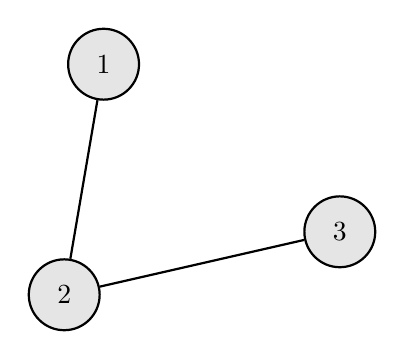
\begin{tikzpicture}
[every node/.style={draw, circle, fill=gray!20!, minimum size=9mm},
thick]
\node(1){1};
\node(2)[below=2cm of 1, xshift=-5mm]{2};
\node(3)[below=1.2cm of 1, xshift=3cm]{3};
\draw (1) -- (2);
\draw (2) -- (3);
\end{tikzpicture}
\end{figure}

\end{flushleft}
 

\paragraph{Constraints:}

\begin{itemize}
\item $1 \leq n \leq 10000$
\item \fcj{wells.length == n}
\item \fcj{0 <= wells[i] <= 10^5}
\item \fcj{1 <= pipes.length <= 10000}
\item \fcj{1 <= pipes[i][0], pipes[i][1] <= n}
\item \fcj{0 <= pipes[i][2] <= 10^5}
\item \fcj{pipes[i][0] != pipes[i][1]}
\end{itemize}

\subsection{Minimum Spanning Tree}
This is a typical Minimum Spanning Tree problem, except that at each node, we have the option of digging new wells.

The trick here is to view \textit{digging new wells} as \textit{laying new pipes to a hidden well 0}. Then we have a typical \textbf{MST} problem to solve.

We use Kruskal algorithm using a disjoint set. The pseudocode of this algorithm is as below

\setcounter{lstlisting}{0}
\begin{lstlisting}[style=customc, caption={Kruskal's Algorithm}]
vector<Edge> kruskal( vector<Edge> edges, int numVertices )
{
    DisjSets ds{ numVertices };
    priority_queue pq{ edges };
    vector<Edge> mst;
    while( mst.size( ) != numVertices - 1 )
    {
        Edge e = pq.pop( ); // Edge e = (u, v)
        SetType uset = ds.find( e.getu( ) );
        SetType vset = ds.find( e.getv( ) );
        if( uset != vset )
        {
            // Accept the edge
            mst.push_back( e );
            ds.union( uset, vset );
        }
    }
    return mst;
}
\end{lstlisting}

In the implementation, we first change each \fcj{wells} into a \fcj{pipe} which is the cost from each node to a dummy node 0 and add to the input array \fcj{pipes}.

The priority queue is not needed here since we can sort the pipes inplace.
\begin{lstlisting}[style=customc, caption={MST By Kruskal}]
int minCostToSupplyWater( int n, vector<int>& wells, vector<vector<int>>& pipes )
{
    int node = 1;
    //change each well into a pipe
    //which connect node to a dummy house 0
    //and then insert into pipes
    for( int well : wells )
    {
        pipes.emplace_back( vector<int> {0, node++, well} );
    }
    //sort pipes inplace per the cost
    sort( begin( pipes ), end( pipes ), []( const vector<int>& p1, const vector<int>& p2 )
    {
        return p1[2] < p2[2];
    } );
    //the vectors used for DSU
    vector<int> parents( n + 1ll );
    for( int i = 0; i <= n; ++i )
    {
        parents[i] = i;
    }
    vector<int> ranks( n + 1ll );
    int ans = 0;
    //Kruskal's algorithm
    for( const auto& edge : pipes )
    {
        int x = edge[0];
        int y = edge[1];
        auto px = find( x, parents );
        auto py = find( y, parents );
        if( px != py )
        {
            //we ignore add x and y into MST
            //since the problem doesn't need
            ans += edge[2];
            //connect x and y
            connect( px, py, parents, ranks );
        }
    }
    return ans;
}
//union find
int find( int x, vector<int>& parents )
{
    while( x != parents[x] )
    {
        x = parents[x];
    }

    return x;
}
//connect x and y with path compression
void connect( int x, int y, vector<int>& parents, vector<int>& ranks )
{
    auto px = find( x, parents );
    auto py = find( y, parents );
    if( px != py )
    {
        if( ranks[px] < ranks[py] )
        {
            std::swap( px, py );
        }
        else if( ranks[px] == ranks[py] )
        {
            ++ranks[px];
        }
        parents[py] = px;
    }
}
\end{lstlisting}
\end{document}
